% Édition critique numérique des diagrammes astronomiques

\subsection{Définir les pratiques de l'édition de diagrammes géométriques}
	Dans un article publié en 2010, Boris et Nicholas Jardin soulignent la disparité des pratiques d'édition des textes et des diagrammes dans l'édition critique de textes canoniques\footcite{jardineCriticalEditingEarlyModern2010}. Dans le domaine de l'histoire des sciences, où se pose particulièrement cette question de l'édition des diagrammes qui accompagnent le texte, les auteurs soulignent l'existence d'éditions critiques qualitatives de textes canoniques, dans lesquelles les diagrammes reproduits sont altérés pour correspondre au contenu du texte, délaissant ainsi la fidélité à la source historique. La critique de cette pratique émane essentiellement du constat suivant :
	
	\begin{displayquote}
		Ils ont effectués ces changements sans commentaire, une démarche qu'aucun d'entre eux n'aurait seulement envisagé de faire avec le texte [Traduction libre].\footnote{\textit{\og they had made those changes without comment, something none of them would have thought of doing with the text \fg}. \cite{jardineCriticalEditingEarlyModern2010}}
	\end{displayquote}
    
    Pensés comme simple accompagnement des textes scientifiques, les diagrammes sont édités en tant qu'outil de compréhension du discours pour un lecteur contemporain, délaissant ainsi l'aspect historique et la richesse en termes de tradition des textes qu'ils peuvent porter. Face aux ressources lacunaires quant à la définition des pratiques d'édition des diagrammes, Jardine et Jardine soulèvent des problématiques assimilables à celles de l'édition critique des textes du point de vue de la gestion des erreurs et des variations, et de la modification des conventions au fil de l'histoire. 
    
    Ainsi, cette perception des diagrammes comme simple outil d'illustration du texte est remise en question, notamment dans les travaux d'Eastwood sur l'astronomie médiévale\footcite{eastwoodPlanetaryDiagramsRoman2004}, qui soulignent l'utilité des diagrammes comme support de compréhension, d'interprétation et de réinterprétation des textes, et argumente qu'une étude poussée des diagrammes présents dans les sources historiques permet une compréhension nouvelle des textes scientifiques : au-delà de simples illustrations, ils sont une clé d'analyse des idées et des théories scientifiques\footcite{jardineCriticalEditingEarlyModern2010}. En tant que nouvel objet d'étude, les diagrammes géométriques se placent comme élément d'intérêt pour l'établissement de la tradition d'un texte : dans un article publié en 2013, Dominique Raynaud souligne le fait que les erreurs présentes dans les diagrammes peuvent éventuellement \og faciliter la distinction et la hiérarchisation de manuscrits d'une même oeuvre [Traduction personnelle]\footnote{\textit{\og Therefore, diagrams make it easier to discriminate between and sort the manuscripts of a given work. \fg}\cite{raynaudBuildingStemmaCodicum2014}} \fg , renforçant cette idée de la nécessité d'éditions critiques qualitatives, qui rendent compte des erreurs et évolutions de ces représentations.
    
    L'édition critique des diagrammes est, pour l'historien, un enjeu scientifique récent, et les pratiques éditoriales dans ce domaine restent mouvantes, loin d'un cadre établit par une norme globale. De la reproduction stricte à la correction des erreurs, les choix de représentation des diagrammes appartiennent à l'éditeur : pour faire du diagramme un objet d'étude au même titre que le texte, ces derniers se doivent d'être considérés comme des sources historiques à part entière. L'ambivalence des besoins en termes de reproduction des diagrammes, de support de compréhension du texte à objet d'étude à part entière, rend complexes les choix binaires nécessaires à l'édition papier d'un texte. Dans ce contexte, l'édition numérique se présente comme une solution possible, qui redéfinit les limites de l'édition critique.
    
    \subsection{Édition critique numérique : pratiques, perspectives et limites}
        \subsubsection{Outils numériques pour l'édition critique}
		\begin{displayquote}
			Nous sommes certainement à l'aube de changements conséquents dans les pratiques éditoriales. De ce fait, il semble probable que la diffusion de l'édition numérique réduise la tension entre l'édition axée sur l'origine [des diagrammes] et celle axée sur la réception [Traduction personnelle]\footnote{\textit{\og 			We are surely on the verge of further very substantial shifts in editorial practice. Thus it seems likely that the spread of digital editions will reduce the tension between origin-focused and reception-focused editing. \fg}. \cite{jardineCriticalEditingEarlyModern2010}}
		\end{displayquote}
	
		Boris et Nicholas Jardine soulignent, en conclusion de l'article précédemment cité, la transformation du paysage éditorial amorcée par la diffusion et la normalisation de l'édition numérique. Dans la continuité des questionnements liés à l'édition critique de diagrammes géométriques et aux limites de l'édition papier pour leur exploitation, le numérique se présente comme une solution potentielle aux choix tranchés que le support impose aux éditeurs. Jardine et Jardine envisage ainsi, sans mise en pratique, la possibilité d'éditions numériques qui rendent compte du rôle historique des illustrations dans la diffusion des idées et dans la pratique scientifique\footcite{jardineCriticalEditingEarlyModern2010}.
		
		En pratique, les solutions pour les éditions critiques numériques sont nombreuses, et présentent également leurs propres limites techniques, tout en étant parfois méconnues des chercheurs\footcite{apollonDigitalCriticalEditions2014} et appliquées sans uniformité entre les projets d'édition. L'enjeu, ainsi, porte également sur l'intégration des outils numériques aux pratiques de l'édition critique et de la philologie\footcite{apollonDigitalCriticalEditions2014}, et particulièrement dans le cadre de l'édition de diagrammes géométriques, qui se développe à l'origine dans un cadre peu défini. Les solutions appliquées, sans universalité, dépendent ainsi des compétences et pratiques des acteurs des projets, et les choix faits en termes d'outil varient profondément d'une édition à l'autre. Ainsi, si des initiatives diverses ont vu le jour pour la définition de normes et de standards pour l'édition numérique\footnote{Ces initiatives sont souvent axées sur le texte : nous pouvons notamment évoquer la \acrfull{tei}, standard basé sur le \acrshort{xml}, qui vise à définir une norme pour la représentation numérique du texte par la publication de guides d'encodage.}, les projets restent libres dans leur procédé éditorial\footcite{apollonDigitalCriticalEditions2014}.
		
		Dans ce contexte, et face à l'existence d'un grand nombre d'outils pour l'édition critique du texte, il n'existe pas de normes numériques pour l'édition des diagrammes géométriques\footnote{Dans ce contexte, nous employons le termes d'\og édition \fg pour décrire la transformation d'un diagramme existant au format papier -- ou en tant qu'image numérique d'une source -- en objet informatique manipulable pour l'analyse, la publication, ou l'édition numérique.}, et leur transformation en objets informatiques s'appuie souvent sur l'adaptation d'outils et de pratiques dédiés aux textes et réadaptés à ces sources visuelles. À titre d'exemple, l'Académie des Sciences de Berlin-Brandenburg mène depuis 1919 un projet -- toujours en cours -- d'édition critique monumentale de l'œuvre de Gottfried Wilhelm Leibniz. En 2009, l'édition prend un tournant digital sous la forme du projet Leibniz-Online\footcite{LeibnizOnlineLeibnizEditionc}, qui a fait le choix du langage \LaTeX en tant qu'outil pour l'édition numérique. \LaTeX étant un outil dédié à la mise en forme de documents, les fonctionnalités adaptées à l'édition critique de textes sont nombreuses ; pour les diagrammes, nombreux dans les textes de Leibniz et transcrits à partir des diagrammes manuscrits présents dans les sources primaires, Leibniz-Online fait le choix d'une exécution en \LaTeX également, en adaptant des \textit{packages} existant pour la création de schéma (fig. \ref{fig:leibniz_diag}). Les diagrammes transcrits sont rendus disponibles au format PDF dans un dépôt GitHub contenant le code de l'édition\footcite{TelotaLeibnizVIIILaTeX_TEIa}, et existent ainsi en tant qu'objets informatiques dans un format peu manipulable, figé après compilation. La transcription en \LaTeX de ces diagrammes est une étape manuelle effectuée par les éditeurs du projets, et représente une tâche particulièrement chronophage du processus d'édition\footnote{Ces explications sont basées sur une présentation donnée par l'équipe du projet Leibniz-Online à l'occasion d'une rencontre organisée par le projet ERC Adg PHILIUMM (laboratoire SPHERE) à l'Université de Paris.}. Les diagrammes encodés en \LaTeX emploient de nouvelles commandes créées pour les besoins spécifiques d'une édition, qui ne s'alignent donc sur aucun standard qui en assurerait l'intéropérabilité. Le projet d'édition critique de l'œuvre de Leibniz est, à ce jour, en cours depuis plus de cent ans : il se pose ainsi la question de la pérennité du code et de la transmission des pratiques de transcription. 
		
		\begin{figure}[h]
			\centering
			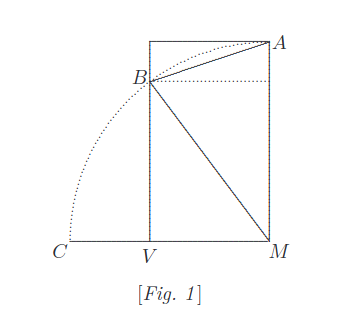
\includegraphics[width=15cm]{images/leibniz_diag.png}
			\caption{Diagrammes extraits de l'édition numérique de l'œuvre complet de Leibniz, volume VIII, 3, p. 665}
			\label{fig:leibniz_diag}
		\end{figure}
	
		En l'absence de norme pour l'édition numérique des diagrammes, les projets ont la liberté de sélectionner les outils, méthodes et formats employés, créant ainsi un paysage disparate de la transcription des diagrammes géométriques, sans pratiques communes et uniformes entre les différents projets. La transcription de ces diagrammes sous forme d'objets informatiques en vue de leur édition est souvent une étape chronophage, manuelle, faisant appel à des outils qu'il est nécessaire pour les chercheurs de prendre en main\footnote{On peut citer, à titre d'exemple, le logiciel libre GeoGebra qui, s'il n'est pas destiné à l'édition, permet la création de diagrammes numériques dans des formats divers. \cite{GeoGebra}}.
		
		Face à cette absence de solution numériques uniformes pour la transcription des diagrammes géométriques, l'\ia intervient comme une solution à la copie manuelle de diagrammes pour leur transformation en objet informatique depuis la source primaire. L'application à l'édition de diagrammes d'algorithmes de vectorisation permet de considérer une automatisation de chaînes de traitement à ce jour essentiellement manuelle, et de penser le développement d'outils libres destinés à l'édition qui définiraient des pratiques systématiques pour la création de versions numériques de diagrammes géométriques.

        \subsubsection{Définition des pratiques pour les diagrammes astronomiques}
        L'existence d'une interface numérique pour l'analyse de diagrammes présente un nombre d'avantages face à leur édition papier, limitée d'un point de vue matériel, et forçant l'éditeur à des choix qui ne correspondent pas nécessairement aux besoins d'un projet de recherche. Les versions numérisées de diagrammes géométriques permettent des actions pour l'analyse qui transcendent les limites physiques des sources historiques : il est ainsi possible d'envisager une comparaison de diagrammes par superposition, qui permettrait de souligner les évolutions d'un même diagramme dans les différentes versions d'une œuvre, d'enrichir les transcriptions de métadonnées pour en expliciter les éléments et choix éditoriaux, ou de faciliter la fouille de corpus de diagrammes, de leur appliquer des manipulations diverses, et de proposer une assistance à l'édition numérique des éléments visuels de textes scientifiques. Ces perspectives rendent cruciale la création d'interfaces pour l'étude et le traitement des diagrammes, à l'image des possibilités, outils et méthodes existants pour l'édition numérique du texte.
        
        Le projet \eida a pour ambition de créer une plateforme destinée à l'édition des diagrammes astronomiques, intégrant la vision artificielle pour proposer des fonctionnalités de transcription automatique. En amont du développement des plateformes et de l'entraînement d'algorithmes de vectorisation, la question des modalités d'édition des diagrammes se pose -- en lien avec les chercheurs, toujours dans une optique de répondre à leurs besoins et de produire des plateformes qui serviront leurs travaux -- pour définir les pratiques qui influenceront la création des outils. Trois types d'édition, c'est-à-dire de transcription à partir d'une image scannée d'un diagramme, sont envisagés : l'édition diplomatique, qui reproduit fidèlement le diagramme sur l'image en incluant ses erreurs, l'édition recalculée, qui prend en compte des paramètres encore à définir pour produire une version corrigée du diagramme, ou une édition critique, qui met en parallèle différentes versions d'un même diagramme pour en souligner les différences. Ces trois types d'éditions présentent un intérêt dans le cadre des recherches effectuées sur ces sources historiques, de l'étude de la circulation des idées à l'analyse de la pratique scientifique dans un contexte historique donné. L'emploi d'algorithmes de vision artificielle permet, à ce jour, de trancher en faveur d'une édition diplomatique, qui transcrirait à l'identique le diagramme soumis. La vectorisation sans correction est, en effet, ce que permet à ce jour la technique ; ainsi, comme mentionné dans les chapitres précédents, il est nécessaire de trouver un équilibre entre les attentes des chercheurs et les possibilités de ce type d'algorithme de vision.
